\documentclass[conference]{IEEEtran}
\usepackage{bm}
\usepackage{cite}
\usepackage{ragged2e}
\usepackage{graphicx}
\usepackage{amsmath}
\usepackage{amssymb}
\usepackage{amsthm}
\usepackage{algorithm}
\usepackage{algpseudocode}
\usepackage{enumitem}
\usepackage{etoolbox}
\usepackage{mathrsfs}
\usepackage[caption=false]{subfig}
\usepackage{array}
\usepackage{cases}
\usepackage{dsfont}
\usepackage{optidef}
\usepackage{cleveref}

\allowdisplaybreaks
\newtheorem{theorem}{Theorem}
\newtheorem{lemma}{Lemma}
\newtheorem{definition}{Definition}
\setlength{\columnsep}{0.21in}
\makeatletter
\newcommand\fs@betterruled{%
  \def\@fs@cfont{\bfseries}\let\@fs@capt\floatc@ruled
  \def\@fs@pre{\vspace*{0.03in}\hrule height.8pt depth0pt \kern2pt}%
  \def\@fs@post{\kern2pt\hrule\relax}%
  \def\@fs@mid{\kern2pt\hrule\kern2pt}%
  \let\@fs@iftopcapt\iftrue}
\floatstyle{betterruled}
\restylefloat{algorithm}
\makeatother
\renewcommand{\arraystretch}{1.2}
\begin{document}
\title{5G DDoS}
\author{\IEEEauthorblockN{Zhan-Lun Chang\IEEEauthorrefmark{1}, Chih-Yu Wang\IEEEauthorrefmark{2}, Hung-Yu Wei\IEEEauthorrefmark{3}}
\IEEEauthorblockA{
\IEEEauthorrefmark{1}\IEEEauthorrefmark{2}Research Center for Information Technology Innovation, Academia Sinica\\
\IEEEauthorrefmark{3}Graduate Institute of Electrical Engineering, National Taiwan University\\
\IEEEauthorrefmark{1}zhc915@citi.sinica.edu.tw,
\IEEEauthorrefmark{2}cywang@citi.sinica.edu.tw,
\IEEEauthorrefmark{3}hywei@ntu.edu.tw,
}}
\maketitle

\begin{abstract}
To be added ... 
\end{abstract}

\section{Introduction}
To be added ... 

\section{Related Works}

\section{System Model}
\begin{figure}[!ht] 
\centering
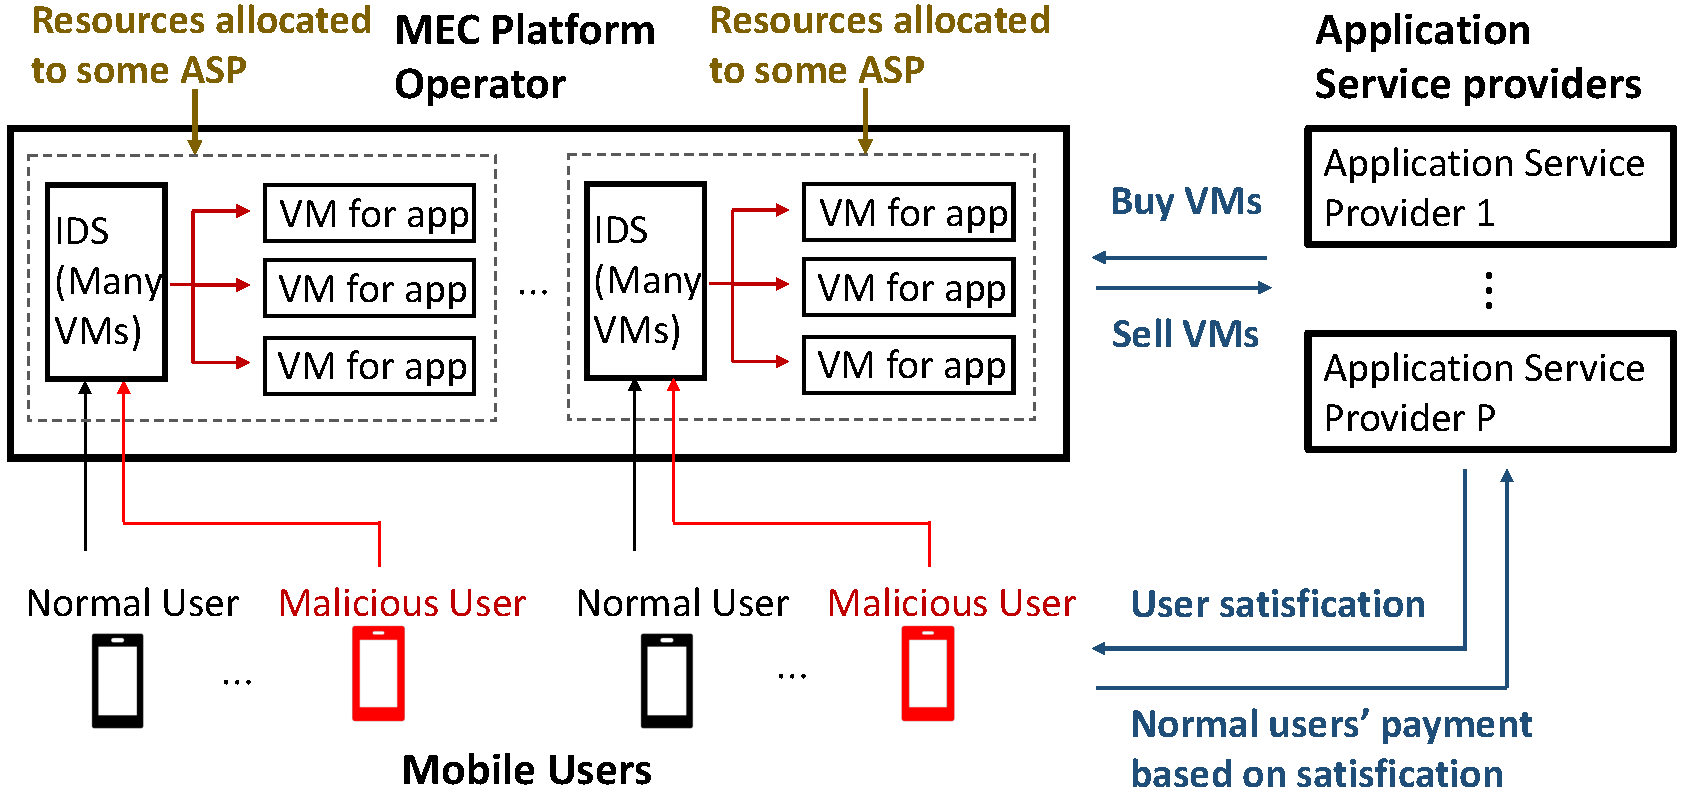
\includegraphics[width= \columnwidth]{5GDDoS_Game_system_architecture.pdf}
\caption{System Architecture}
\label{fig:system}
\end{figure}
We illustrate our system architecture in Fig~\ref{fig:system}. There are three types of entities in our system: the MEC platform operator (MPO), application service providers (ASPs), and end-users (EUs). The MPO manages the computation resources in terms of virtual machines (VMs) of geographically distributed edge servers. Since the ASPs do not have the computation resources to process the application tasks, they have strong demands for the MPO's VMs whose total number is $\mathcal{Q}_{V}$. The goal of the MPO is to maximize its profit by finding the optimal unit selling price $\Psi_{m}^v$ per VM. We denote the set of ASPs as $\mathcal{I}=\{1, \cdots, I\}$. The ASPs determine the number of VMs to buy (denoted by $z_i^v$) from MPO to maximize their profit too. The ASPs utilize these purchased VMs to either run the application service or mitigate the DDoS security attacks. If ASPs devote most of their VMs to running the application service, they are prone to DDoS security attacks. The security threat would damage the users' quality of experience (QoE) and thus the revenue of ASPs. Even worse, it would paralyze the application service such that the ASPs have no revenue. On the other hand, if the ASPs devote most of their VMs to mitigating the DDoS attack, they can not ensure good satisfaction to the users (e.g., users' latency requirements can not be satisfied) even though the ASPs are immune from the DDoS attacks. Therefore, it is crucial to find an optimal resource allocation between running the application service and mitigating the DDoS attacks. We denote the set of EUs associated with ASP $i \in \mathcal{I}$ as $\mathrm{U}_i$ and further categorize it into two kinds: normal users (NUs) $\mathrm{U}_i^n$ and malicious users (MUs) $\mathrm{U}_i^m$. Each MU $j \in \mathrm{U}_i$ has the Poisson task arrival rate $\lambda_{ij}$, latency requirement $d_{ij}$, and task size $s_{ij}$. We consider the situation that the EUs do not have enough computation resources or needed resources such as Graphics Processing Unit (GPU) resources to process the application tasks. Therefore, they will offload the tasks out to the MPO.  

The DDoS attacks happen when the AUs flood into the edge servers. The ASPs can intercept some malicious requests by employing open-source intrusion prevention system (IPS) such as Suricata \cite{Suricata}. The IPS of all ASPs monitors and filters all task requests, and all VMs devoted to running the application service process the filtered task requests. We assume the IPS does not classify the normal task requests as malicious, but it can not discern all malicious requests and would classify some malicious task requests as normal. How many malicious requests can the IPS filter depends on how many VMs the ASPs dedicate to the IPS. We use $H(\cdot)$ to represent the relationship between the quantity of intercepted malicious requests and the number of devoted VMs. $H(\cdot)$ is assumed to be nondecreasing and concave. Also, $H(0)=0$. In this paper, we recommend a linear function form of $H(x) = \eta{x}$ so that the closed form solutions can be derived in the following optimization problems. The cost of using IPS only comes from the devoted VMs and does not include any payment because it is open-source.

We consider orthogonal frequency-division multiple access (OFDMA) system and thus the bandwidth of the edge servers whose computation resources are allocated to ASP $i$ denoted by $B_i$ can be divided into $|\mathrm{U}_i|$ sub-bands of size $W_{i} = B_i/|\mathrm{U}_i|$. Each MU $j\in \mathrm{U}_i$ transmits the data over each of $|\mathrm{U}_i|$ sub-bands, and hence they would not cause interference to other EUs while transmitting. The maximum achievable uplink data transmission rate $R_{ij}$ between ASP $i$ and MU $j \in \mathrm{U}_i$ is 
\begin{equation} \label{eqn:shannon}
R_{ij}=W_i \cdot log_2\Big(1+\frac{p_{ij}g_{ij}}{N_{0}}\Big)
\end{equation}
where $p_{ij}$ is the maximum transmission power of MU $j$ in $\mathrm{U}_i$, and $g_{ij}$ denotes the uplink channel gain between ASP $i$ and MU $j$. $N_0$ is the background noise power. Based on this rate, we can calculate the mean transmission time of workload consisting of tasks with size $s_{ij}$ from MU $j \in \mathrm{U}_i$ to ASP $i$. 
\begin{equation} 
T_{ij}^t=\frac{\lambda_{ij} \cdot s_{ij}}{R_{ij}}
\end{equation}

The task arrival process at ASP $i$ still follows the Poisson process according to the Poisson process's stationary property. Furthermore, the mean arriving rate of the Poisson process at ASP $i$ can be expressed as $\lambda_i = \sum_{j \in \mathrm{U}_i} \lambda_{ij}$ based on the superposition property of the Poisson process. Since the ASPs buy VMs from MPO whose overall computation resources are still limited compared to the cloud platform such as Google cloud platform or Amazon EC2 platform, we model the meaning processing delay of all VMs purchased by ASPs using $M/M/1$ queue. Each VM of MPO is homogeneous and can process $f_m^v$ CPU cycles per second. As the average required CPU cyles for a task of ASP $i$ may be different, the mean service rate of the queue at ASP $i$ denoted by $\mu_i^v$ (the number of tasks that a VM can process on average per second) is different for every ASP $i$. We denote the required CPU cycles of user $j \in \mathsf{U}_i$ as $\chi_{ij}$. The relationship between $f_m^v$ and $\mu_i^v$ is
\begin{equation}
\mu_i^v = f_m^v/(\frac{\sum_{j \in \mathsf{U}_i} \chi_{ij}}{|\mathrm{U}_i|})
\end{equation}
If the ASP $i$ devotes $z_i^h$ out of $z_i^v$ VMs to IPS, the intercepted quantity of malicious requests is $H(z_i^h)$. When ASP $i$ buys $z_i^v$ VMs from the MPO and devotes $z_i^h$ to IPS, those VMs' mean processing delay is 
\begin{equation} \label{eqn:asp_mm1_delay}
T_i^p(z_i^v, z_i^h) = \frac{1}{(z_i^v - z_i^h)\mu_i^v - \big(\lambda_i - H(z_i^h)\big)}
\end{equation}

The payment from the NU $j \in \mathrm{U}_i^n$ to the ASP $i$ depends on whether the latency requirements $d_{ij} \, \forall j \in \mathrm{U}_i^n$ are satisfied or not. If latency requirements $d_{ij}$ are met, NU $j \in \mathrm{U}_i^n$ pays a price $\Psi_{ij}$ to ASP $i$. The heterogeneity of the payment reflects the different characteristics of NUs. The NUs with different latency requirements may have different level of satisfaction with the same service provided by the ASP $i$. If latency requirements $d_{ij}$ are not met, NU $j \in \mathrm{U}_i^n$ does not pay ASP $i$. The MUs $j \in \mathrm{U}_i^m$ will not pay any money to the ASP $i$ no matter whether their latency requirement are satisfied or not. We represent the payment of EU $j \in \mathrm{U}_i$ as follows:
\begin{subnumcases}{\mathcal{K}_{ij}(z_i^v, z_i^h)=\label{eqn:devicepayment}}
  \Psi_{ij} & \hspace*{-1.7mm}if $T_{ij}^t + T_i^p(z_i^v, z_i^h) \leq d_{ij}$, $j \in \mathrm{U}_i^n$\\
  0 & \hspace*{-1.7mm}if $T_{ij}^t + T_i^p(z_i^v, z_i^h) > d_{ij}$, $j \in \mathrm{U}_i^n$ \\
  0 & \hspace*{-1.7mm}$j \in \mathrm{U}_i^m$
\end{subnumcases}

\section{Game Formulation}
Because of the rationalities of both MPO and ASPs, the intrinsic hierarchy between MPO and ASPs, and the influence of one ASP's action on other ASPs' profits, we model the interaction between MPO and ASPs as a two-stage single-leader-multi-followers Stackelberg game. Both the MPO and ASPs are rational players and have the ultimate goal of maximizing their profits by adjusting their actions. The MPO can select a price per VM $\Psi_{m}^v$ that maximizes its profit, and the ASPs determine how many VMs to buy from MPO $z_i^v \, \forall i$ to maximize its profit too. The MPO's selection of price per VM affects how many VMs those ASPs would buy, which in turn has an impact on the selection of price. Since the ASPs need to buy the computation resources from MPO to maintain their application services, the MPO has an advantage over the ASPs. Moreover, due to MPO's finite number of VMs, the more one ASP buys, the less other ASPs can buy. The action of one ASP affects other ASPs' profit. The Stackelberg game where the MPO acts as the leader and all ASPs are the followers can capture the coupled and hierarchical relationship between MPO and ASPs, the self-interests of both MPO and ASPs, and the implicit influence among ASPs. We illustrate the actions and utilities of MPO and ASPs in the following first and then formulate the optimization problems for both players. 

\subsection{The Action and The Utility of ASPs}
Given the MPO's price per VM $\Psi_m^v$, each ASP $i$ chooses how many VMs to buy from the MPO $z_i^v$ to maximize its profit which is the revenue accrued from the normal MU $j \in \mathrm{U}_i^n$ minus the payment to the MPO for purchasing $z_i^v$ VMs. The natural candidate for the utility is the profit. However, even with the same $z_i^v$, the revenue of ASP $i$ hinges on how many VMs it dedicates to the IPS, distribution of latency requirements $d_{ij}$, and the different payments of heterogeneous NU $j \in \mathrm{U}_i^n$. We define the utility of ASP $i$ when it purchases $z_i^v$ VMs from MPO as the maximum expected profit across the different number of VMs dedicates to the IPS $z_i^h$ with respect to the distribution of latency requirement $d_{ij}$. Furthermore, to make the optimization problem tractable, we assume that the latency requirements $d_{ij} \, \forall j \in \mathrm{U}_i$ are drawn from the same uniform distribution indexed by $i$ over interval $[a_i, b_i]$ denoted by $\mathcal{U}(a_i,b_i)$ and relax the variables of ASPs $z_i^v, z_i^h \, \forall i \in \mathcal{I}$ to real numbers. The utility of ASP $i$ given $\Psi_m^v$ is
\begin{align}
&Y_i(z_i^v|\Psi_m^v) \triangleq \max_{z_i^h} \mathsf{E}_{d_{ij}}\Big[\sum_{j \in \mathrm{U}_i^n} \mathcal{K}_{ij}(z_i^v, z_i^h) - \Psi_m^v z_i^v\Big] \\ 
&\hspace*{-1mm}=\max_{z_i^h} \mathsf{E}_{d_{ij}}[\sum_{j \in \mathrm{U}_i^n}\Psi_{ij}\mathds{1}\{T_{ij}^t + T_i^p(z_i^v, z_i^h) \leq d_{ij}\} - \Psi_m^vz_i^v] \nonumber \\ 
&\hspace*{-1mm}=\max_{z_i^h} [\sum_{j \in \mathrm{U}_i^n}\Psi_{ij}(1-\frac{T_{ij}^t + T_i^p(z_i^v, z_i^h)-a_i}{b_i-a_i}) - \Psi_m^vz_i^v] \label{eqn:asp_def_subobjective_unfold} \\
&\hspace*{-1mm}\triangleq \max_{z_i^h} X_i(z_i^h|z_i^v,\Psi_m^v) \label{eqn:asp_def_subobjective}
\end{align}
$\mathsf{E}_{d_{ij}}$ means taking expectation with respect to the distribution of $d_{ij}$, and $\mathds{1}\{\cdot\}$ is the indicator function. Given $z_i^v$, we have two constraints on $z_i^h$. First, the number of VMs dedicated to IPS $z_i^h$ must be no larger than the number of purchased VMs $z_i^v$. Second, to make the processing queue stable, the mean service rate by the VMs dedicated to running the service must be higher than the mean arrival rate for EUs $j \in \mathrm{U}_i$. To define the utility of ASP $i$ when the purchased VMs from the MPO is $z_i^v$, we have to solve the following optimization problem. 
\begin{maxi!}[2]
  {z_i^h \in \mathbb{R}}
  {X_i(z_i^h|z_i^v,\Psi_m^v) \label{eqn:asp_utility_def_opti_obj}}
  {\label{eqn:asp_utility_def_opti}}
  {}
  \addConstraint{0 \leq z_i^h \leq \xi_i z_i^v}{\label{eqn:asp_utility_def_opti_const1}}
  \addConstraint{\phi_i z_i^v \mu_i^v \leq (z_i^v-z_i^h)\mu_i^v - \lambda_i + H(z_i^h) }{\label{eqn:asp_utility_def_opti_const2}}
\end{maxi!}
In (\ref{eqn:asp_utility_def_opti_const1}), we further introduce a system parameter $\xi_i$ to control the feasible range of $z_i^h$. Similarly, in (\ref{eqn:asp_utility_def_opti_const2}), we use another system parameter $\phi_i$ to specify the quantity by which the mean service rate must exceed the mean arrival rate. The observation that both (\ref{eqn:asp_utility_def_opti_const1}) and (\ref{eqn:asp_utility_def_opti_const2}) impose upper bounds on the range of $z_i^h$ will simplify the characterization of the optimal $z_i^h$. Showing the utility of the ASP $i$, $Y_i(z_i^v)$, is well-defined is equivalent to proving the optimization problem (\ref{eqn:asp_utility_def_opti}) has at lease one solution. If there are multiple optimal points that have the same values of $X_i(z_i^h|z_i^v,\Psi_m^v)$, we randomly select one to be the solution to (\ref{eqn:asp_utility_def_opti}).
\begin{lemma}
The utility of ASP $i$, $Y_i(z_i^v)$, is well defined. That is, the optimization problem (\ref{eqn:asp_utility_def_opti}) has at least one optimal point. Moreover, the optimization problem (\ref{eqn:asp_utility_def_opti}) is a convex optimization problem.
\end{lemma}
\begin{proof}
The feasible region imposed by (\ref{eqn:asp_utility_def_opti_const1}) and (\ref{eqn:asp_utility_def_opti_const2}) is a closed and bounded interval in $\mathbb{R}$ and thus is a convex set. As the objective function (\ref{eqn:asp_utility_def_opti_obj}) is continuous in $z_i^h$, the existence of the optimal solution then comes from the Extreme Value Theorem. If (\ref{eqn:asp_utility_def_opti_obj}) is concave at each feasible $z_i^h$, optimization problem (\ref{eqn:asp_utility_def_opti}) is a convex optimization problem. It remains to show that the objective function (\ref{eqn:asp_utility_def_opti_obj}) is concave in feasible $z_i^h$. By rearranging the terms, we express $X_i(z_i^h|z_i^v,\Psi_m^v)$ as 
\begin{equation}
\sum_{j \in \mathrm{U}_i^n}\Psi_{ij}(1-\frac{T_{ij}^t -a_i}{b_i-a_i})- \Psi_m^v z_i^v - \sum_{j \in \mathrm{U}_i^n}\Psi_{ij}(\frac{T_i^p(z_i^v, z_i^h)}{b_i-a_i})
\end{equation}
 To show $X_i(z_i^h|z_i^v,\Psi_m^v)$ is concave in feasible $z_i^h$, it suffices to show that $T_i^p(z_i^v, z_i^h)$ is convex in feasible $z_i^h$. We verity the concavity of $T_i^p(z_i^v, z_i^h)$ by taking second derivative with respect to $z_i^h$. 
\begin{subequations}\label{eqn:asp_subobjective_second_deriv}
     \begin{alignat}{1}
       &[(z_i^v- z_i^h)\mu_i^v - \lambda_i + H(z_i^h)]^{-3} \cdot [-\mu_i^v+H'(z_i^h)]^2 \label{eqn:asp_subobjective_second_deriv_first_term} \\
       &+ (-1) \cdot [(z_i^v-z_i^h)\mu_i^v - \lambda_i + H(z_i^h)]^{-2} \cdot H''(z_i^h) \label{eqn:asp_subobjective_second_deriv_second_term}
     \end{alignat}
\end{subequations}
$H'(z_i^h)$ and $H''(z_i^h)$ stand for first and second derivative with respect to $z_i^h$. In (\ref{eqn:asp_subobjective_second_deriv_first_term}) and (\ref{eqn:asp_subobjective_second_deriv_second_term}), $(z_i^v- z_i^h)\mu_i^v - \lambda_i - H(z_i^h)$ is always positive at each feasible $z_i^h$ because of (\ref{eqn:asp_utility_def_opti_const2}). Also, as $H(\cdot)$ is concave, $H''(z_i^h)$ is non-positive. Therefore, (\ref{eqn:asp_subobjective_second_deriv_first_term}) and (\ref{eqn:asp_subobjective_second_deriv_second_term}) are non-negative. We can conclude that the second derivative of $T_i^p(z_i^v, z_i^h)$ is non-negative, and $T_i^p(z_i^v, z_i^h)$ is convex in feasible $z_i^h$. 
\end{proof}
After defining the utility of ASP $i$, $Y_i(z_i^v)$, we can now formulate the optimization problem of ASP $i$ given the MPO's price per VM $\Psi_m^v$. 
\begin{maxi!}[2]
  {z_i^v \in \mathbb{R}}
  {Y_i(z_i^v|\Psi_m^v) \label{eqn:asp_utility_opti_obj}}
  {\label{eqn:asp_utility_opti}}
  {}
  \addConstraint{\lambda_i+ \gamma_i \leq z_i^v \mu_i^v}{\label{eqn:asp_utility_opti_const1}}
  \addConstraint{0 \leq Y_i(z_i^v|\Psi_m^v)}{\label{eqn:asp_utility_opti_const2}}
\end{maxi!}
The constraint (\ref{eqn:asp_utility_opti_const1}) regulates that when the ASP $i$ dedicates all purchased VMs to running the application service, the mean service rate must be larger than the mean arrival rate by at least $\gamma_i$. (\ref{eqn:asp_utility_opti_const1}) also ensures that the feasible region of (\ref{eqn:asp_utility_def_opti}) is non-empty because under this constraint, there is at least one $z_i^h$ that satisfies (\ref{eqn:asp_utility_def_opti_const2}). The constraint (\ref{eqn:asp_utility_opti_const2}) represents the individual rationality for every ASP. That is, when making the processing queue stable gives a negative utility, the ASPs would rather choose not to serve the users' requests and do not buy any VMs from the MPO, which has zero utility. We defer the analysis of solutions to both optimization problems (\ref{eqn:asp_utility_def_opti}) and (\ref{eqn:asp_utility_opti}) to the \Cref{sec:game_optimization}. We denote the solution to (\ref{eqn:asp_utility_opti}) as $(z_i^v(\Psi_m^v))^*$ to emphasize the dependence on the MPO's price per VM $\Psi_m^v$. 

\subsection{The Action and The Utility of The MPO}
With the prediction about the number of VMs purchased by ASPs $(z_i^v(\Psi_m^v))^* \, \forall i \in \mathcal{I}$, the MPO chooses the price per VM $\Psi_m^v$ to maximize its utility which is defined as the MPO's profit. The revenue of the MPO is the sum of payments from all ASPs. Although the ASPs buy the VMs from the MPO, it is the infrastructure of the MPO that processes the application requests. As a result, the MPO has an operating cost for keeping the VMs working. We represent the cost for operating $\sum_{i \in \mathcal{I}} (z_i^v(\Psi_m^v))^*$ VMs by $C_m^v\big(\sum_{i \in \mathcal{I}} (z_i^v(\Psi_m^v))^*\big)$. The function $C_m^v(\cdot)$ is assumed to be convex and non-decreasing, which means that both the marginal cost and the cost increase as the number of VMs that the MPO has to keep running increases. We denote the MPO's utility as $Y_m(\Psi_m^v)$ and formulate the MPO's optimization problem.
\begin{maxi!}[2]
  {\Psi_m^v}
  {\Psi_m^v \cdot \sum_{i \in \mathcal{I}} (z_i^v(\Psi_m^v))^* - C_m^v\big(\sum_{i \in \mathcal{I}} (z_i^v(\Psi_m^v))^*\big) \label{eqn:mpo_utility_opti_obj}} 
  {\label{eqn:mpo_utility_opti}}
  {}
  \addConstraint{\sum_{i \in \mathcal{I}} (z_i^v(\Psi_m^v))^* \leq \mathcal{Q}_v}{\label{eqn:mpo_utility_opti_const1}}
  \addConstraint{0 \leq \Psi_m^v}{\label{eqn:mpo_utility_opti_const2}}
\end{maxi!}
The constraint (\ref{eqn:mpo_utility_opti_const1}) mandates that the MPO can not sell more VMs than the total number of VMs $\mathcal{Q}_v$ that the MPO has. The constraint (\ref{eqn:mpo_utility_opti_const1}) imposes a lower bound for MPO's price per VM. The constraint (\ref{eqn:mpo_utility_opti_const2}) requires the MPO's price per VM must be non-negative. The property of this optimization (\ref{eqn:mpo_utility_opti}) relies on the solution $(z_i^v(\Psi_m^v))^*$, and we defer the analysis to \Cref{sec:game_optimization}.
\section{Game Optimization} \label{sec:game_optimization}
We would leverage the backward induction principle to solve the formulated Stackelberg game. In this principle, we solve the followers' (ASPs') optimization problems first and then the leader's (the MPO's) optimization problem based on responses of ASPs to the MPO's price per VM, i.e., $(z_i^v(\Psi_m^v))^* \, \forall i \in \mathcal{I}$. Before delving into the solution process, we first define the Stackelberg game equilibrium. We symbolize the ASP $i$'s action set using $\mathcal{A}_i$ and the profile of all ASPs' action using $\bm{z^v}=(z_1^v, z_2^v, \cdots, z_I^v) \in \mathcal{A}_1 \times \mathcal{A}_2 \cdots \times \mathcal{A}_I$ where $\mathcal{A}_1 \times \mathcal{A}_2$ means the Cartesian product of $\mathcal{A}_1$ and $\mathcal{A}_2$. The ASP $i$'s best response set $\mathcal{B}_i^R(\Psi_m^v)$ to the MPO's price per VM $\Psi_m^v$ is given by 
\begin{equation} \label{eqn:asp_best_response}
\begin{aligned}
\mathcal{B}_i^R(\Psi_m^v) = &\{z_i^v \in \mathcal{A}_i |Y_i(z_i^v|\Psi_m^v) \geq Y_i\big((z_i^v)'|\Psi_m^v\big) \\
&\forall (z_i^v)' \in \mathcal{A}_i, (z_i^v)' \neq z_i^v\}
\end{aligned}
\end{equation}
We also denote the Cartesian product of all ASPs' best response sets as
\begin{equation}
\mathcal{B}^R(\Psi_m^v) = \mathcal{B}_1^R(\Psi_m^v) \times \mathcal{B}_2^R(\Psi_m^v) \cdots \times \mathcal{B}_I^R(\Psi_m^v)
\end{equation}
Likewise, we denote the MPO's action set as $\mathcal{A}_m$. Furthermore, to stress the influence of ASPs' actions on the MPO's utility, we use $Y_m(\Psi_m^v|\bm{z^v})$ to represent the MPO's utility in the following definition of the MPO's best response set.
\begin{equation} \label{eqn:mpo_best_response}
\begin{aligned}
\mathcal{B}_m = &\{\Psi_m^v \in \mathcal{A}_m| Y_m(\Psi_m^v|\bm{z^v}) \geq Y_m((\Psi_m^v)'|(\bm{z^v})') \\
&\forall (\Psi_m^v)' \in \mathcal{A}_m, (\Psi_m^v)' \neq \Psi_m^v, \forall \bm{z^v} \in \mathcal{B}^R(\Psi_m^v) \\
&\forall  (\bm{z^v})' \in \mathcal{B}^R\big((\Psi_m^v)'\big)\}
\end{aligned}
\end{equation}
\begin{definition}[\textbf{Stackelberg equilibrium}] \label{def:stackelberg_equilibrium}
If $\mathcal{B}_{m}$ and $\mathcal{B}^R(\Psi_m^v)$ are both non-empty, the Stackelberg equilibrium in our mechanism is a vector of dimension $(I+1)$ that is an element of $\mathcal{B}_m  \times \mathcal{B}^R(\Psi_m^v)$.
\end{definition}
We analyze the solution process of the formulated Stackelberg game according to whether the solution to (\ref{eqn:asp_utility_def_opti}) is the extreme point or boundary point of the constraint. 

\textbf{Case 1}: The optimal point of (\ref{eqn:asp_utility_def_opti}) is the extreme point whose first derivative with respect to $z_i^h$. The first derivative of $X_i(z_i^h|z_i^v,\Psi_m^v)$ with respect to $z_i^h$ is
\begin{equation} \label{eqn:asp_utilitu_def_firstderiv}
[(z_i^v - z_i^h) - \lambda_i + H(z_i^h)]^{-2} \cdot (-\mu_i^v + H'(z_i^h))
\end{equation}
$(z_i^v - z_i^h) - \lambda_i + H(z_i^h)$ is positive at every feasible $z_i^h$ because of the constraint (\ref{eqn:asp_utility_def_opti_const2}). Also, $H'(\cdot)$ is non-decreasing and thus has an inverse function denoted by $G(\cdot)$. We can solve the extreme point denoted by $(z_i^h)^*$ through letting (\ref{eqn:asp_utilitu_def_firstderiv}) equal zero. 
\begin{equation} \label{eqn:asp_utility_def_extreme_point}
(z_i^h)^* = (H')^{-1}(\mu_i^v) \triangleq G(\mu_i^v)
\end{equation}
When we substitute (\ref{eqn:asp_utility_def_extreme_point}) into (\ref{eqn:asp_mm1_delay}), the mean processing delay denoted as $T_{i,1}^p(z_i^v)$ depends only on $z_i^v$ and is 
\begin{equation}
T_{i,1}^p(z_i^v) = \frac{1}{\big(z_i^v - G(\mu_i^v)\big)\mu_i^v - \lambda_i + H\big(G(\mu_i^v)\big)}
\end{equation}
According to (\ref{eqn:asp_def_subobjective_unfold}) and (\ref{eqn:asp_def_subobjective}), the objective function (\ref{eqn:asp_utility_opti_obj}) becomes
\begin{equation}\label{eqn:asp_case1_utility}
Y_i^1(z_i^v|\Psi_m^v) \triangleq \sum_{j \in \mathrm{U}_i^n}\Psi_{ij}(1-\frac{T_{ij}^t + T_{i,1}^p(z_i^v)-a_i}{b_i-a_i}) - \Psi_m^vz_i^v
\end{equation}
If we optimize (\ref{eqn:asp_case1_utility}), we can observe how the ASP reacts to different $z_i^v$ and $\Psi_m^v$ in order to reach the highest utility. However, we won't try to do so since the case doesn't happen based on the initial assumption of $H(x) = \eta{x}$. We briefly explain the property in the following.
\begin{lemma} \label{lemma:asp_case1_not_exist}
$X_1(z_i^h|z_i^v,\Psi_m^v)$ doesn't have extreme point in feasible $z_i^h$ if $H(x) = \eta{x}$.
\end{lemma}
\begin{proof}  
From (\ref{eqn:asp_utilitu_def_firstderiv}),  we substitute $\eta{z_i^h}$ into $H(z_i^h)$, then we can obtain
\begin{equation} \label{eqn:asp_utilitu_simplified}
[(z_i^v - z_i^h) - \lambda_i + \eta{z_i^h}]^{-2} \cdot (-\mu_i^v + \eta)
\end{equation}
Obviously, no matter what the value of $z_i^h$ is, (\ref{eqn:asp_utilitu_simplified}) equaling zero will never be satisfied. Therefore, the extreme point of (\ref{eqn:asp_case1_utility}) does not exist.
Now we know that the extreme point of (\ref{eqn:asp_utility_def_opti_obj}) does not exist in feasible $z_i^h$, so the maximum value of $X_1(z_i^h|z_i^v,\Psi_m^v)$ only happens at the boundary points of feasible $z_i^h$.
\qedhere
\end{proof}
\textbf{Case 2}: The optimal point of (\ref{eqn:asp_utility_def_opti}) happens at the right boundary of (\ref{eqn:asp_utility_def_opti_const1}). That is, when the purchased number of VM is $z_i^v$, the ASP $i$'s optimal number of VMs devoted to the IPS is
\begin{equation} \label{eqn:asp_utility_def_first_boundary}
(z_i^h)^* = \xi_i z_i^v
\end{equation}
When we substitute (\ref{eqn:asp_utility_def_first_boundary}) into (\ref{eqn:asp_mm1_delay}), the mean processing delay in this case denoted as $T_{i,2}^p(z_i^v)$ is
\begin{equation} \label{eqn:asp_case2_mm1_delay}
T_{i,2}^p(z_i^v) =  \frac{1}{(1-\xi_i)z_i^v\mu_i^v - \big(\lambda_i - H(\xi_iz_i^v)\big)}
\end{equation}
according to (\ref{eqn:asp_def_subobjective_unfold}) and (\ref{eqn:asp_def_subobjective}), the objective function (\ref{eqn:asp_utility_opti_obj}) becomes
\begin{equation} \label{eqn:asp_case2_objective}
Y_i^2(z_i^v|\Psi_m^v) \triangleq \sum_{j \in \mathrm{U}_i^n}\Psi_{ij}(1-\frac{T_{ij}^t + T_{i,2}^p(z_i^v)-a_i}{b_i-a_i}) - \Psi_m^vz_i^v
\end{equation}
If $Y_i^2(z_i^v|\Psi_m^v)$ is concave in feasible $z_i^v$, it is much easier to solve the optimization problem (\ref{eqn:asp_utility_opti}) with the objective being $Y_i^2(z_i^v|\Psi_m^v)$. We prove this properties in the following. 
\begin{lemma} \label{lemma:asp_case2_utility_concave}
$Y_i^2(z_i^v|\Psi_m^v)$ is concave in feasible $z_i^v$.
\end{lemma}
\begin{proof}
If $T_{i,2}^p(z_i^v)$ is convex in feasible $z_i^v$, $Y_i^2(z_i^v|\Psi_m^v)$ is concave in feasible $z_i^v$. We can verify the convexity of $T_{i,2}^p(z_i^v)$ by taking second derivative of $T_{i,2}^p(z_i^v)$ with respect to $z_i^v$. 
\begin{equation} \label{eqn:asp_case2_mm1_delay_second_deriv}
\begin{aligned}
&2[(1-\xi_i)\mu_i^v z_i^v - \lambda_i + H(\xi_i z_i^v)]^{-3}\times [(1-\xi_i)\mu_i^v\\
&+ \xi_i H'(\xi_i z_i^v)]^2-[(1-\xi_i)\mu_i^v z_i^v - \lambda_i + H(\xi_i z_i^v)]^{-2}  \\
& \times (\xi_i)^2 H''(\xi_i z_i^v)
\end{aligned}{}
\end{equation}
Since $(z_i^h)^* = \xi_i z_i^v$ satisfies the constraint (\ref{eqn:asp_utility_def_opti_const2}), $(1-\xi_i)\mu_i^v z_i^v - \lambda_i + H(\xi_i z_i^v)$ is always positive. Moreover, as $H(\cdot)$ is concave, $H''(\xi_i z_i^v)$ is non-positive. The first term of (\ref{eqn:asp_case2_mm1_delay_second_deriv}) is positive, and the second term of (\ref{eqn:asp_case2_mm1_delay_second_deriv}) is non-positive. Therefore, (\ref{eqn:asp_case2_mm1_delay_second_deriv}) is non-negative, which means $T_{i,2}^p(z_i^v)$ is convex in feasible $z_i^v$. Hence, $Y_i^2(z_i^v|\Psi_m^v)$ is concave in feasible $z_i^v$. \qedhere
\end{proof}
With \Cref{lemma:asp_case2_utility_concave}, we can characterize the solution to the optimization problem (\ref{eqn:asp_utility_opti}) when the objective function (\ref{eqn:asp_utility_opti_obj}) equals $Y_i^2(z_i^v|\Psi_m^v)$ in the following theorem with a specific form of $H(\cdot)$. Before stating the result, we define the feasible region of (\ref{eqn:asp_utility_opti_const1}) as $\Upsilon_i$ for ASP i while the feasible region of (\ref{eqn:asp_utility_opti_const2}) as $\Upsilon_i^2$ when the $Y_i(z_i^v|\Psi_m^v)$ equals $Y_i^2(z_i^v|\Psi_m^v)$. 
\begin{theorem}\label{thm:asp_case2_optimal}
The solution to the optimization problem (\ref{eqn:asp_utility_opti}) when the objective function (\ref{eqn:asp_utility_opti_obj}) equals $Y_i^2(z_i^v|\Psi_m^v)$ and $H(x)=\eta x$ is $(z_{i,2}^v(\Psi_m^v))^*$ 
\begin{subnumcases}{=\label{eqn:asp_case2_optimal_solution}}
  0 & if $\Upsilon_i \cap \Upsilon_i^2 = \emptyset$ \label{eqn:asp_case2_optimal_solution_individual_rationality} \\
  \frac{\lambda_i+\gamma_i}{\mu_i} & if $\Upsilon_i \cap \Upsilon_i^2 \neq \emptyset $ and $(z_{i,2}^{v,e}(\Psi_m^v))^* < \frac{\lambda_i+\gamma_i}{\mu_i}$ \label{eqn:asp_case2_optimal_solution_lower_boundary} \\ 
  (z_{i,2}^{v,e}(\Psi_m^v))^* & if $\Upsilon_i \cap \Upsilon_i^2 \neq \emptyset $ and $(z_{i,2}^{v,e}(\Psi_m^v))^* \geq \frac{\lambda_i+\gamma_i}{\mu_i}$ \label{eqn:asp_case2_optimal_solution_extreme} 
\end{subnumcases}
where
\begin{equation}\label{eqn:asp_case2_utility_extreme}
\begin{aligned} 
(z_{i,2}^{v,e}(\Psi_m^v))^* &= \sqrt{\frac{\sum_{j \in \mathrm{U}_i^n}\Psi_{ij}}{(b_i-a_i)\Psi_m^v [(1-\xi_i)\mu_i^v + \xi_i \eta]}} \\
&+ \frac{\lambda_i}{(1-\xi_i)\mu_i^v + \xi_i \eta}
\end{aligned}
\end{equation}
\end{theorem}
\begin{proof}
We begin by proving the feasible region is a convex set. $\Upsilon_i$ is a convex set because $\Upsilon_i$ is a ray starting from $\frac{\lambda_i+\gamma_i}{\mu_i}$ to $\infty$. Since we have proved the convexity of $Y_i^2(z_i^v|\Psi_m^v)$ in \Cref{lemma:asp_case2_utility_concave}, $\Upsilon_i^2$ is a convex set because any superlevel set of a concave function is a convex set. Since the intersection of two convex set is a convex set, $\Upsilon_i \cap \Upsilon_i^2$ is a convex set. When $\Upsilon_i \cap \Upsilon_i^2 = \emptyset$, which means the ASP $i$ cannot make the processing queue stable while has a positive utility no matter how many VMs ASP $i$ buys from the MPO. In this situation, the best action of ASP $i$ is not to buy any VM. By \Cref{lemma:asp_case2_utility_concave}, $Y_i^2(z_i^v|\Psi_m^v)$ is concave. When the extreme point of $Y_i^2(z_i^v|\Psi_m^v)$ is smaller than $\frac{\lambda_i+\gamma_i}{\mu_i}$, $\frac{\lambda_i+\gamma_i}{\mu_i}$ is the optimal point. When the extreme point of $Y_i^2(z_i^v|\Psi_m^v)$ falls in the interior of the feasible region, the extreme point is the optimal point. The extreme point of $Y_i^2(z_i^v|\Psi_m^v)$ can be solved when the first derivative of $Y_i^2(z_i^v|\Psi_m^v)$ with respect to $z_i^v$ equals zero.
\begin{equation} \label{eqn:asp_case2_utility_first_deriv}
-\frac{\partial T_{i,2}^p(z_i^v)}{\partial z_i^v} = \frac{\Psi_m^v (b_i - a_i)}{\sum_{j \in \mathsf{U}_i^n} \Psi_{ij}}
\end{equation}
Using (\ref{eqn:asp_case2_mm1_delay}), (\ref{eqn:asp_case2_objective}), and $H(x)=\eta x$, it only takes simple algebraic operations to have the expression for the extreme point in (\ref{eqn:asp_case2_utility_extreme}). \qedhere
\end{proof}

From \Cref{thm:asp_case2_optimal}, we can obtain the MPO's price per VM $\Psi_m^i$ which makes the ASP $i$'s optimal response switch among (\ref{eqn:asp_case2_optimal_solution_individual_rationality}), (\ref{eqn:asp_case2_optimal_solution_lower_boundary}) and (\ref{eqn:asp_case2_optimal_solution_extreme})by solving the $\Psi_m^v$ that satisfies $Y_i^2(\frac{\lambda_i+\gamma_i}{\mu_i}|\Psi_m^v) = 0$ and $(z_{i,2}^{v,e}(\Psi_m^v))^* = \frac{\lambda_i+\gamma_i}{\mu_i}$. 
\begin{equation} 
\begin{aligned}
\Psi_{m,2}^{i,z}&= \frac{\sum_{j \in \mathrm{U}_i^n}\Psi_{ij}}{(b_i-a_i)[(1-\xi_i)\mu_i^v + \xi_i \eta]} \\
& \times \big[\frac{\lambda_i+\gamma_i}{\mu_i} - \frac{\lambda_i}{(1-\xi_i)\mu_i^v + \xi_i\eta}\big]^{-2} 
\end{aligned} 
\end{equation}.
\begin{equation} 
\begin{aligned}
\Psi_{m,2}^{i,l}&= \sum_{j \in \mathrm{U}_i^n}\Psi_{ij}(1-\frac{T_{ij}^t + T_{i,1}^p(z_i^v)-a_i}{b_i-a_i}) \\
& \times \big[\frac{\lambda_i+\gamma_i}{\mu_i} - \frac{\lambda_i}{(1-\xi_i)\mu_i^v + \xi_i\eta}\big]^{-2} \times (\frac{\mu_i}{\lambda_i+\gamma_i})
\end{aligned}
\end{equation}
\iffalse
The $z_i^v$ will switch from $0$ to $\frac{\lambda_i+\gamma_i}{\mu_i}$ at $\Psi_{m,2}^{i,z}$ and $\frac{\lambda_i+\gamma_i}{\mu_i}$ to$(z_{i,2}^{v,e}(\Psi_m^v))^*$ at $\Psi_{m,2}^{i,l}$.
\fi
Based on the analysis above, the MPO can predict how many VMs every ASP will buy given an arbitrary price of VM when $(z_i^h)^* = \xi_i z_i^v$.

\textbf{Case 3}: The optimal point of (\ref{eqn:asp_utility_def_opti}) happens at the boundary of (\ref{eqn:asp_utility_def_opti_const2}). That is, when the purchased number of VM is $z_i^v$, the ASP $i$'s optimal number of VMs devoted to the IPS $(z_i^h)^*$ satisfies
\begin{equation} \label{eqn:asp_utility_def_second_boundary}
\phi_i z_i^v \mu_i^v = \big(z_i^v-(z_i^h)^*\big)\mu_i^v - \lambda_i + H\big((z_i^h)^*\big)
\end{equation}
When we substitute (\ref{eqn:asp_utility_def_second_boundary}) into (\ref{eqn:asp_mm1_delay}), the mean processing delay denoted as $T_{i,3}^p(z_i^v)$ depends only on $z_i^v$ and is 
\begin{equation}
T_{i,3}^p(z_i^v) = \frac{1}{\phi_i z_i^v \mu_i^v}
\end{equation}
According to (\ref{eqn:asp_def_subobjective_unfold}) and (\ref{eqn:asp_def_subobjective}), the objective function (\ref{eqn:asp_utility_opti_obj}) becomes
\begin{equation}
Y_i^3(z_i^v|\Psi_m^v) \triangleq \sum_{j \in \mathrm{U}_i^n}\Psi_{ij}(1-\frac{T_{ij}^t + T_{i,3}^p(z_i^v)-a_i}{b_i-a_i}) - \Psi_m^vz_i^v
\end{equation}
If $Y_i^3(z_i^v|\Psi_m^v)$ is concave in feasible $z_i^v$, it is much easier to solve the optimization problem (\ref{eqn:asp_utility_opti}) with the objective being $Y_i^3(z_i^v|\Psi_m^v)$. We prove this properties in the following. 
\begin{lemma} \label{lemma:asp_case3_utility_concave}
$Y_i^3(z_i^v|\Psi_m^v)$ is concave in feasible $z_i^v$.
\end{lemma}
\begin{proof}
If $T_{i,3}^p(z_i^v)$ is convex in feasible $z_i^v$, $Y_i^3(z_i^v|\Psi_m^v)$ is concave in feasible $z_i^v$. We can verify the convexity of $T_{i,3}^p(z_i^v)$ by taking second derivative of $T_{i,3}^p(z_i^v)$ with respect to $z_i^v$
\begin{equation} \label{eqn:asp_case3_mm1_delay_second_deriv}
\frac{\partial^2 T_{i,3}^p(z_i^v)}{\partial (z_i^v)^2} = 2(z_i^v)^{-3}\frac{1}{\phi_i \mu_i^v} \geq 0 
\end{equation}
The second derivative (\ref{eqn:asp_case3_mm1_delay_second_deriv}) is always non-negative, which means $T_{i,3}^p(z_i^v)$ is convex in feasible $z_i^v$. Hence, $Y_i^3(z_i^v|\Psi_m^v)$ is concave in feasible $z_i^v$.
\end{proof}
We characterize the solution to the optimization problem (\ref{eqn:asp_utility_opti}) when the objective function (\ref{eqn:asp_utility_opti_obj}) equals $Y_i^3(z_i^v|\Psi_m^v)$ in the following theorem. Before stating the result, we define the feasible region of (\ref{eqn:asp_utility_opti_const2}) as $\Upsilon_i^3$ when the $Y_i(z_i^v|\Psi_m^v)$ equals $Y_i^3(z_i^v|\Psi_m^v)$. When $\Upsilon_i \cap \Upsilon_i^3$ is an non-empty interval in $\mathbb{R}^+$, we express the left endpoint of $\Upsilon_i \cap \Upsilon_i^3$ as $\zeta_i^{3l}$ and the right endpoint of $\Upsilon_i \cap \Upsilon_i^3$ as $\zeta_i^{3u}$.
\begin{theorem}\label{thm:asp_case3_optimal}
The solution to the optimization problem (\ref{eqn:asp_utility_opti}) when the objective function (\ref{eqn:asp_utility_opti_obj}) equals $Y_i^3(z_i^v|\Psi_m^v)$ is 
$(z_{i,2}^v(\Psi_m^v))^*$ 
\begin{subnumcases}{=\label{eqn:asp_case3_optimal_solution}}
  0 & if $\Upsilon_i \cap \Upsilon_i^3 = \emptyset$ \label{eqn:asp_case3_optimal_solution_individual_rationality} \\
  \zeta_i^{3l} & if $(z_{i,3}^{v,e}(\Psi_m^v))^* < \zeta_i^{3l}$ \label{eqn:asp_case3_optimal_solution_lower_boundary} \\ 
  \zeta_i^{3u} & if $(z_{i,3}^{v,e}(\Psi_m^v))^* > \zeta_i^{3u}$ \label{eqn:asp_case3_optimal_solution_upper_boundary} \\
  (z_{i,3}^{v,e}(\Psi_m^v))^* & if $(z_{i,3}^{v,e}(\Psi_m^v))^* \in (\zeta_i^{3l}, \zeta_i^{3u})$ \label{eqn:asp_case3_optimal_solution_extreme} 
\end{subnumcases}
where
\begin{equation} \label{eqn:asp_case3_utility_extreme}
(z_{i,3}^{v,e}(\Psi_m^v))^* = \sqrt{\frac{\sum_{j \in \mathrm{U}_i^n}\Psi_{ij}}{\phi_i \mu_i^v(b_i-a_i)\Psi_m^v}} 
\end{equation}
\end{theorem}
\begin{proof}
We begin by proving the feasible region is a convex set. $\Upsilon_i$ is a convex set because $\Upsilon_i$ is a ray. Since we have proved the convexity of $Y_i^3(z_i^v|\Psi_m^v)$ in \Cref{lemma:asp_case3_utility_concave}, $\Upsilon_i^3$ is a convex set because any superlevel set of a concave function is a convex set. Since the intersection of two convex set is a convex set, $\Upsilon_i \cap \Upsilon_i^3$ is a convex set. When $\Upsilon_i \cap \Upsilon_i^3 = \emptyset$, which means the ASP $i$ cannot make the processign queue stable while has a positive utility no matter how many VMs ASP $i$ buys from the MPO. In this situation, the best action of ASP $i$ is not to buy any VM. By \Cref{lemma:asp_case3_utility_concave}, $Y_i^3(z_i^v|\Psi_m^v)$ is concave. When the extreme point of $Y_i^3(z_i^v|\Psi_m^v)$ is smaller than $\zeta_i^{3l}$, $\zeta_i^{3l}$ is the optimal point. Likewise, when the extreme point of $Y_i^3(z_i^v|\Psi_m^v)$ is larger than $\zeta_i^{3u}$, $\zeta_i^{3u}$ is the optimal point. When the extreme point of $Y_i^3(z_i^v|\Psi_m^v)$ falls in the interior of the feasible region, the extreme point is the optimal point. The extreme point of $Y_i^3(z_i^v|\Psi_m^v)$ can be solved when the first derivative of $Y_i^3(z_i^v|\Psi_m^v)$ with respect to $z_i^v$ equals zero.
\begin{equation} \label{eqn:asp_case3_utility_first_deriv}
-\frac{\partial T_{i,2}^p(z_i^v)}{\partial z_i^v} = (z_i^v)^{-2}\frac{1}{\phi_i \mu_i^v}=\frac{\Psi_m^v (b_i-a_i)}{\sum_{i \in \mathrm{U}_i^n}\Psi_{ij}}
\end{equation}
It only takes simple algebraic operations to have the expression for the extreme point in (\ref{eqn:asp_case3_utility_extreme}).\qedhere
\end{proof}
From \Cref{thm:asp_case3_optimal}, we can obtain the MPO's price per VM $\Psi_m^i$ which makes the ASP $i$'s optimal response switch among (\ref{eqn:asp_case3_optimal_solution_lower_boundary}), (\ref{eqn:asp_case3_optimal_solution_upper_boundary}), and (\ref{eqn:asp_case3_optimal_solution_extreme}) by solving the $\Psi_m^v$ that satisfies $(z_{i,3}^{v,e}(\Psi_m^v))^* = \zeta_i^{3l}$ or $(z_{i,3}^{v,e}(\Psi_m^v))^* = \zeta_i^{3u}$. 
\begin{equation}
\begin{aligned}
\Psi_{m,3}^{i,l} = \frac{\sum_{j \in \mathrm{U}_i^n}\Psi_{ij}}{\phi_i \mu_i^v(b_i-a_i)}\big(\zeta_i^{3u}\big)^2 \\
\Psi_{m,3}^{i,u} = \frac{\sum_{j \in \mathrm{U}_i^n}\Psi_{ij}}{\phi_i \mu_i^v(b_i-a_i)}\big(\zeta_i^{3l}\big)^2 \\
\end{aligned}
\end{equation}
The sequence $\{\Psi_{m,3}^{i,l} , \Psi_{m,3}^{i,u}, \forall i \in \mathcal{I}\}$ partitions the space of the MPO's price per VM $\Psi_m^v$ into $2I + 1$ intervals.
\begin{equation}
0 \cup \mathbb{R}^{+} = \mathcal{M}_3^1 \cup \mathcal{M}_3^1 \cdots \cup \mathcal{M}_3^{2I+1}
\end{equation}
Within each interval $\mathcal{M}_3^k, \forall k \in \{1, \cdots, 2I+1\}$, we define four sets of ASP $i$ that has different optimal responses.
\begin{equation}
\begin{aligned}
&\Omega_3^{k,z} = \{i \in \mathcal{I}|(z_{i,3}^v(\Psi_m^v))^* = 0\} \\
&\Omega_3^{k,l} = \{i \in \mathcal{I}|(z_{i,3}^v(\Psi_m^v))^* = \zeta_i^{3l}\} \\
&\Omega_3^{k,u} = \{i \in \mathcal{I}|(z_{i,3}^v(\Psi_m^v))^* = \zeta_i^{3u}\} \\
&\Omega_3^{k,e} = \{i \in \mathcal{I}|(z_{i,3}^v(\Psi_m^v))^* = (z_{i,3}^{v,e}(\Psi_m^v))^*\} 
\end{aligned}
\end{equation}
These four sets form a partition of the all ASPs. That is, $\mathcal{I} = \Omega_3^{k,z} \cup \Omega_3^{k,l} \cup \Omega_3^{k,u} \cup \Omega_3^{k,e}, \, \forall k \in \{1, \cdots, 2I+1\}$. The total number of VMs bought by the ASPs within each interval $\mathcal{M}_2^k, \forall k \in \{1, \cdots, 2I+1\}$ can be expressed 
\begin{equation}\label{eqn:asp_case3_total_number_VM}
\sum_{i \in \mathcal{I}} (z_{i,3}^v(\Psi_m^v))^* =  \sum_{i\in \Omega_3^{k,l}}\zeta_i^{3l} + \sum_{i\in \Omega_3^{k,u}}\zeta_i^{3u} + \sum_{i \in \Omega_3^{k,e}}(z_{i,3}^{v,e}(\Psi_m^v))^* 
\end{equation}
With the expression (\ref{eqn:asp_case3_total_number_VM}), the MPO's optimization problem in each interval $\mathcal{M}_3^k, \forall k \in \{1, \cdots, 2I+1\}$ is
\begin{maxi!}[2]
  {\Psi_m^v}
  {\Psi_m^v \cdot \sum_{i \in \mathcal{I}} (z_{i,3}^v(\Psi_m^v))^* - C_m^v\big(\sum_{i \in \mathcal{I}} (z_{i,3}^v(\Psi_m^v))^*\big) \label{eqn:case3_mpo_utility_opti_obj}} 
  {\label{eqn:case3_mpo_utility_opti}}
  {}
  \addConstraint{\sum_{i \in \mathcal{I}} (z_{i,3}^v(\Psi_m^v))^* \leq \mathcal{Q}_v}{\label{eqn:case3_mpo_utility_opti_const1}}
  \addConstraint{\Psi_m^v \in \mathcal{M}_3^k}{\label{eqn:case3_mpo_utility_opti_const2}}
\end{maxi!}
\begin{theorem} \label{thm:mpo_case3_convex_optimization}
In each interval $\mathcal{M}_3^k, \forall k \in \{1, \cdots, 2I+1\}$, the MPO's optimization problem (\ref{eqn:mpo_utility_opti}) is a convex optimization problem. The MPO's otpimal price per VM $\Psi_m^v$ is one of the optimal prices in each $\mathcal{M}_3^k, \forall k \in \{1, \cdots, 2I+1\}$ that gives the highest utility. 
\end{theorem}
\begin{proof}
We start by proving that $\sum_{i \in \mathcal{I}} (z_{i,3}^v(\Psi_m^v))^*$ is convex in $\Psi_m^v$ when $\Psi_m^v \in \mathcal{M}_3^k,\, \forall k \in \mathcal{I}$. In (\ref{eqn:asp_case2_total_number_VM}), only the second term pertains to $\Psi_m^v$. As the summation of convex function is also a convex function, it suffices to prove that $(z_{i,3}^v(\Psi_m^v))^*$ is convex in $\Psi_m^v$ for $i \in \Omega_3^{k,e}$. Taking the second derivative of (\ref{eqn:asp_case3_utility_extreme}) with respect to $\Psi_m^v$, we have 
\begin{equation}
\frac{3}{4}(\Psi_m^v)^{-5/2}\sqrt{\frac{\sum_{j \in \mathrm{U}_i^n}\Psi_{ij}}{\phi_i \mu_i^v(b_i-a_i)}}  \geq 0 
\end{equation}
Hence, $(z_{i,3}^v(\Psi_m^v))^*$ is convex in $\Psi_m^v \in \mathcal{M}_3^k,\, \forall k \in \{1,\cdots, 2I+1\}$. Since the sublevel set of a convex function is a convex set, the feasible region resulting from (\ref{eqn:case3_mpo_utility_opti_const1}) is a convex set for any value $\mathcal{Q}_v$. In addition, the feasible region of (\ref{eqn:case3_mpo_utility_opti_const2}) is also a convex set because the convex combination of two numbers in $\mathcal{M}_3^k, \forall k \in \{1, \cdots, 2I+1\}$ is still a number in $\mathcal{M}_3^k, \forall k \in \{1, \cdots, 2I+1\}$. Hence, the feasible region of the optimization problem (\ref{eqn:case3_mpo_utility_opti}) is the intersection of two convex set and thus is a convex set. To prove that the MPO's the optimization problem (\ref{eqn:case3_mpo_utility_opti}) is a convex optimization problem, what remains to do is to prove that the objective function (\ref{eqn:case3_mpo_utility_opti_obj}) is concave in $\Psi_m^v \in \mathcal{M}_3^k,\, \forall k \in \{1,\cdots, 2I+1\}$. Using (\ref{eqn:asp_case3_utility_extreme}) and (\ref{eqn:asp_case3_total_number_VM}), we can unfold the first term in (\ref{eqn:case3_mpo_utility_opti_obj}) as follows. 
\begin{align} \label{eqn:mpo_case3_utility_first_term}
&\Psi_m^v \cdot \sum_{i \in \mathcal{I}} (z_{i,3}^v(\Psi_m^v))^* \\
&= \Psi_m^v\sum_{i\in \Omega_3^{k,l}}\zeta_i^{3l} + \Psi_m^v\sum_{i\in \Omega_3^{k,u}}\zeta_i^{3u} + \sum_{i \in \Omega_3^{k,u}}\Psi_m^v(z_{i,3}^{v,e}(\Psi_m^v))^* \nonumber\\
& = \Psi_m^v (\sum_{i\in \Omega_3^{k,l}}\zeta_i^{3l} + \sum_{i\in \Omega_3^{k,u}}\zeta_i^{3u}) +\sum_{i \in \Omega_3^{k,u}} \sqrt{\frac{\Psi_m^v\sum_{j \in \mathrm{U}_i^n}\Psi_{ij}}{\phi_i \mu_i^v(b_i-a_i)}}  \nonumber
\end{align}
The first term in the final expression (\ref{eqn:mpo_case3_utility_first_term}) is a linear function of $\Psi_m^v$ which is both convex and concave. The second term in the final expression $(\ref{eqn:mpo_case3_utility_first_term})$ is concave in $\Psi_m^v$. To see this, we check the concavity via the second order test. The second derivative of the second term is 
\begin{equation}
 -\frac{1}{4}(\Psi_m^v)^{-3/2}\sum_{i \in \Omega_3^{k,u}} \sqrt{\frac{\sum_{j \in \mathrm{U}_i^n}\Psi_{ij}}{\phi_i \mu_i^v(b_i-a_i)}} \leq 0 
\end{equation}
Therefore, (\ref{eqn:mpo_case3_utility_first_term}) is concave in $\Psi_m^v$. The second term of (\ref{eqn:case3_mpo_utility_opti_obj}), $C_m^v\big(\sum_{i \in \mathcal{I}} (z_{i,3}^v(\Psi_m^v))^*$, is convex in $\Psi_m^v$ as it is a composition of $C_m^v$ and $\sum_{i \in \mathcal{I}} (z_{i,3}^v(\Psi_m^v)$ where $C_m^v$ is convex and non-decreasing, and $\sum_{i \in \mathcal{I}} (z_{i,3}^v(\Psi_m^v))$ is convex in $\Psi_m^v \in \mathcal{M}_3^k,\, \forall k \in \{1, \cdots, 2I+1\}$. Since a concave function minus a convex function yields a concave function, (\ref{eqn:case3_mpo_utility_opti_obj}) is concave in $\Psi_m^v \in \mathcal{M}_3^k,\, \forall k \in \mathcal{I}$. In sum, the MPO's optimization problem (\ref{eqn:case3_mpo_utility_opti}) in each interval $\mathcal{M}_3^k, \forall k \in \{1, \cdots, 2I+1\}$ is a convex optimization problem. \qedhere
\end{proof}
After analyzing both the followers' and the leader's optimization problems, we can now prove that there are at least one Stackelberg game equilibrium in our system with minor modifications on. We convert all the right open intervals among $\mathcal{M}_1^k$, $\mathcal{M}_2^k$, and $\mathcal{M}_3^k$, $\forall k \in \{1, \cdots, 2I+1\}$ into right close intervals with the right endpoint being the right endpoint of original ones minus small constants $\epsilon_1$, $\epsilon_2$, and $\epsilon_3$. 
\begin{theorem} \label{thm:stackelberg_game_equilibrium}
There are at lease one Stackelberg game equlibrium in our system after the modifications.  
\end{theorem}
\begin{proof}
In Case 1, we have analytical solutions for ASPs' optimal number of VMs to buy from the MPO by \Cref{thm:asp_case1_optimal}. The best response sets for ASPs defined in (\ref{eqn:asp_best_response}) are non-empty. With the optimal responses from the ASPs, the MPO's optimal price per VM $\Psi_m^v$ exists becasue when (\ref{eqn:case1_mpo_utility_opti_const2}) becomes $\Psi_m^v \in \mathcal{M}_1^{k'}$, MPO's optimization problem is a convex optimization problem proved in \Cref{thm:mpo_case1_convex_optimization} with a compact feasible region. Thus, the MPO's best response set definded in (\ref{eqn:mpo_best_response}) is non-empty. By \Cref{def:stackelberg_equilibrium}, there are at least one Stackelberg game equlibrium in Case 1. Similarly, in Case 2, we have analytical solutions for ASPs' optimal number of VMs to buy from the MPO by \Cref{thm:asp_case2_optimal}. The best response sets for ASPs defined in (\ref{eqn:asp_best_response}) are non-empty. With the optimal responses from the ASPs, the MPO's optimal price per VM $\Psi_m^v$ exists becasue becasue when (\ref{eqn:case2_mpo_utility_opti_const2}) becomes $\Psi_m^v \in \mathcal{M}_2^{k'}$, MPO's optimization problem is a convex optimization problem proved in \Cref{thm:mpo_case2_convex_optimization} with a compact feasible region. Thus, the MPO's best response set definded in (\ref{eqn:mpo_best_response}) is non-empty. By \Cref{def:stackelberg_equilibrium}, there are at least one Stackelberg game equlibrium in Case 2. Finally, in Case 3, we have analytical solutions for ASPs' optimal number of VMs to buy from the MPO by \Cref{thm:asp_case3_optimal}. The best response sets for ASPs defined in (\ref{eqn:asp_best_response}) are non-empty. With the optimal responses from the ASPs, the MPO's optimal price per VM $\Psi_m^v$ exists becasue becasue when (\ref{eqn:case3_mpo_utility_opti_const2}) becomes $\Psi_m^v \in \mathcal{M}_3^{k'}$, MPO's optimization problem is a convex optimization problem proved in \Cref{thm:mpo_case3_convex_optimization} with a compact feasible region. Thus, the MPO's best response set definded in (\ref{eqn:mpo_best_response}) is non-empty. By \Cref{def:stackelberg_equilibrium}, there are at least one Stackelberg game equlibrium in Case 3.
\end{proof}
Because of \Cref{thm:mpo_case1_convex_optimization}, \Cref{thm:mpo_case2_convex_optimization}, and \Cref{thm:mpo_case3_convex_optimization}, if the specific form of $C_m^v(\cdot)$ is given, we can solve the exact form of the solution to the MPO's optimization problem. We will select some specific forms for $C_m^v(\cdot)$ in the \Cref{sec:simulation}.
\section{Simulation} \label{sec:simulation} 
\bibliographystyle{IEEEtran}
\bibliography{5GDDoS_Game}

\end{document}


